% Generated by tools/golden_study/plot_qft96_checkpoint.py; do not edit by hand.
\begin{figure}[H]
\centering
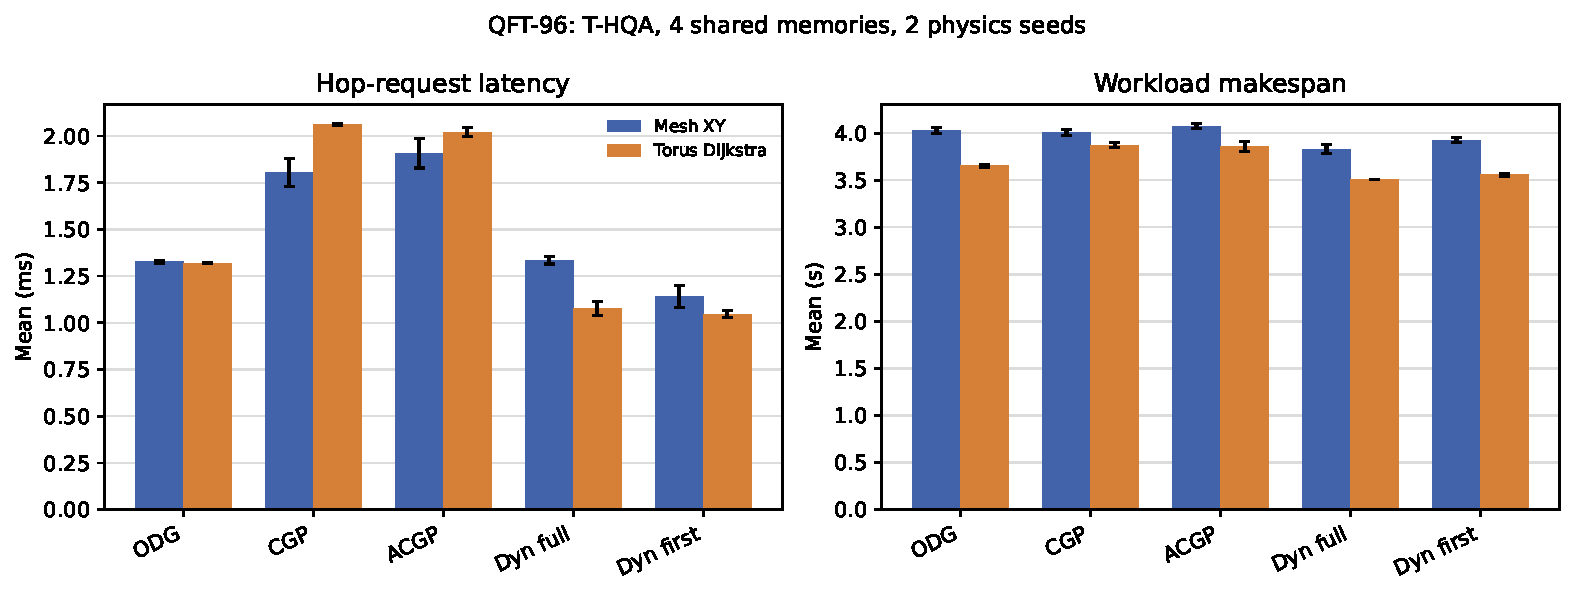
\includegraphics[width=0.9\linewidth]{../../../results/qft96_2seed_2026-10-26/figures/qft96_m4_checkpoint.pdf}
\caption{Validated QFT-96 four-memory checkpoint. Bars show means and standard deviations across physics seeds 0 and 1, not uncertainty across mapping placements. Mesh XY and torus Dijkstra use the same logical migration endpoints. Exact values are in Table~\ref{tab:qft96-m4-timing} and the \href{https://github.com/sanjeevkrishnaa/Compiler-Driven-ACE/blob/codex/ace-scheduler-correctness/results/qft96_2seed_2026-10-26/summaries/qft96_m4_checkpoint.csv}{aggregate CSV}; \href{https://github.com/sanjeevkrishnaa/Compiler-Driven-ACE/blob/codex/ace-scheduler-correctness/results/qft96_2seed_2026-10-26/summaries/qft96_m4_seed_rows.csv}{per-seed rows} are also archived.}
\label{fig:qft96-m4-checkpoint}
\end{figure}
\begin{table}[H]
\centering\scriptsize
\begin{tabular}{llrrrr}
\toprule
Route & Policy & Latency (ms) & p95 (ms) & Makespan (s) & Admission (ms) \\
\midrule
Mesh XY & ODG & 1.327 $\pm$ 0.006 & 3.100 & 4.033 $\pm$ 0.031 & 0.008 \\
Mesh XY & CGP & 1.803 $\pm$ 0.075 & 5.150 & 4.006 $\pm$ 0.031 & 1.043 \\
Mesh XY & ACGP & 1.908 $\pm$ 0.079 & 5.600 & 4.075 $\pm$ 0.028 & 1.149 \\
Mesh XY & Dyn full & 1.335 $\pm$ 0.020 & 4.050 & 3.830 $\pm$ 0.048 & 0.551 \\
Mesh XY & Dyn first-hop & 1.141 $\pm$ 0.058 & 2.900 & 3.928 $\pm$ 0.029 & 0.125 \\
Torus Dijkstra & ODG & 1.320 $\pm$ 0.002 & 3.000 & 3.654 $\pm$ 0.013 & 0.004 \\
Torus Dijkstra & CGP & 2.061 $\pm$ 0.006 & 5.400 & 3.874 $\pm$ 0.024 & 1.223 \\
Torus Dijkstra & ACGP & 2.021 $\pm$ 0.023 & 5.300 & 3.855 $\pm$ 0.054 & 1.199 \\
Torus Dijkstra & Dyn full & 1.075 $\pm$ 0.037 & 2.900 & 3.509 $\pm$ 0.000 & 0.328 \\
Torus Dijkstra & Dyn first-hop & 1.046 $\pm$ 0.019 & 2.700 & 3.557 $\pm$ 0.013 & 0.132 \\
\bottomrule
\end{tabular}
\caption{Complete matched timing values for Figure~\ref{fig:qft96-m4-checkpoint}. ODG has $C=0$; other policies have $C=3$. Latency and makespan show mean $\pm$ sample SD across two physics seeds. The full precision and raw job identifiers are in the \href{https://github.com/sanjeevkrishnaa/Compiler-Driven-ACE/blob/codex/ace-scheduler-correctness/results/qft96_2seed_2026-10-26/summaries/qft96_m4_checkpoint.csv}{source CSV}.}
\label{tab:qft96-m4-timing}
\end{table}
\begin{table}[H]
\centering\scriptsize
\begin{tabular}{llrrr}
\toprule
Route & Policy & Pre-generated hit rate & Protocol waste (\%) & Fidelity \\
\midrule
Mesh XY & ODG & N/A & N/A & 0.9498 \\
Mesh XY & CGP & N/A & 15.07 & 0.9271 \\
Mesh XY & ACGP & N/A & 15.27 & 0.9262 \\
Mesh XY & Dyn full & 0.602 & 0.00 & 0.9438 \\
Mesh XY & Dyn first-hop & 0.340 & 0.00 & 0.9472 \\
Torus Dijkstra & ODG & N/A & N/A & 0.9498 \\
Torus Dijkstra & CGP & N/A & 19.74 & 0.9311 \\
Torus Dijkstra & ACGP & N/A & 19.14 & 0.9307 \\
Torus Dijkstra & Dyn full & 0.656 & 0.00 & 0.9440 \\
Torus Dijkstra & Dyn first-hop & 0.455 & 0.00 & 0.9462 \\
\bottomrule
\end{tabular}
\caption{Readiness, waste and delivered-pair fidelity for the same validated checkpoint; ODG has no pre-generated cache. \href{https://github.com/sanjeevkrishnaa/Compiler-Driven-ACE/blob/codex/ace-scheduler-correctness/results/qft96_2seed_2026-10-26/summaries/qft96_m4_checkpoint.csv}{Source CSV}.}
\label{tab:qft96-m4-quality}
\end{table}
